\chapter{Evaluación experimental}
\label{capitulo3}
\lhead{Capítulo 3. \emph{Evaluación experimental}}

\section{Diseño experimental}

En este capítulo se describen todas las decisiones tomadas con respecto a la experimentación; esto incluye los parámetros usados para la entonación, las particiones hechas en la validación cruzada y la estratificación, el diseño de los experimentos donde se combinan las heurísticas con las metaheurísticas y finalmente se presentan los resultados de cada prueba realizada. 

Lo primero que se hace es entonar los algoritmos evolutivos para que devuelvan el mejor valor posible al probarse con los conjuntos de datos presentados en la sección 2.4. Para lograr la entonación, se usa \emph{irace}, presentado en la sección 2.6, con los parámetros de la tabla \ref{irace-param}. Se consigue una configuración de parámetros para los problemas pequeños, medianos y grandes respectivamente.

\begin{table}[]
\centering
\begin{tabular}{l c}
\hline
Parámetros & irace \\
\hline
\hline
Iteraciones                                 &  1000, 400 y 100\\
Número decimales significativos             &    4            \\
Prueba estadística                          &  t-test         \\
Nivel de significancia para prueba estadística  &  0.05           \\
Frecuencia de la prueba estadística         &    1 iteración  \\
Número de configuraciones élites            &  automática     \\
Reinicialización por convergencia prematura &     Sí          \\
Modo elitista                               &     Sí          \\

\hline
\end{tabular}
\caption{Parámetros usados para \emph{irace}}
\label{irace-param}
\end{table}

Los parámetros a entonar son: número de iteraciones, cardinalidad de la población, probabilidad de cruce, probabilidad de mutación y tamaño del torneo. Los rangos válidos para cada parámetro se presentan en la tabla \ref{rangos}. La elección de los rangos se hace en base a los trabajos \cite{de2004reduccion,de2004reduccion,garcia2012prototype,garcia2008memetic,talbi2009metaheuristics}. Los resultados de la entonación se presentan en las tablas \ref{param-peq}, \ref{param-med} y \ref{param-grande}.

\begin{table}[]
\centering
\begin{tabular}{l c c}
\hline
Parámetros & Tipo de dato & Rangos \\
\hline
\hline

Población                & entero           &  [10,150]       \\
Probabilidad de cruce    & real             &  [0,1]          \\
Probabilidad de mutación & real             &  [0,0.01]      \\
Número del torneo        & entero           &  [1,10]         \\  

\hline
\end{tabular}
\caption{Rangos usados para los parámetros en la entonación}
\label{rangos}
\end{table}

\begin{table}[]
\centering
\begin{tabular}{l c c c c}
\hline
\multirow{2}{*}{\textsc{Parámetros}}
	& \multicolumn{4}{c}{\textsc{Algoritmos}} \\
	& GGA & SGA & MA & CHC \\
\hline
\hline
Iteraciones             &  1000    &  1000    &  1000      &  1000 \\
Población               &    70    &    90    &    21      &    33 \\
Prob. de Cruce          &   0.4837 &   0.9848 &     0.9496 &     - \\
Prob. de Mutación       &   0.0001 &  0.0057  &     0.0071 &     - \\
Número del torneo       &   -      &    3     &     1      &     - \\
\hline
\end{tabular}
\caption{Parámetros usados para los conjuntos pequeños}
\label{param-peq}
\end{table}


\begin{table}[]
\centering
\begin{tabular}{l c c c c}
\hline
\multirow{2}{*}{\textsc{Parámetros}}
	& \multicolumn{4}{c}{\textsc{Algoritmos}} \\
	& GGA & SGA & MA & CHC \\
\hline
\hline
Iteraciones             &  1000    &  1000    &  1000      &  1000 \\
Población               &    88    &    132   &    32      &    27 \\
Prob. de Cruce          &   0.5779 &   0.9859 &     0.9549 &     - \\
Prob. de Mutación       &   0.0001 &  0.0001  &     0.0004 &     - \\
Número del torneo       &   -      &    1     &     3      &     - \\
\hline
\end{tabular}
\caption{Parámetros usados para los conjuntos medianos}
\label{param-med}
\end{table}

\begin{table}[]
\centering
\begin{tabular}{l c c c c}
\hline
\multirow{2}{*}{\textsc{Parámetros}}
	& \multicolumn{4}{c}{\textsc{Algoritmos}} \\
	& GGA & SGA & MA & CHC \\
\hline
\hline
Iteraciones             &  1000    &  1000    &  1000      &  1000 \\
Población               &    102   &    122   &    35      &    37 \\
Prob. de Cruce          &   0.5158 &   0.9554 &     0.9698 &     - \\
Prob. de Mutación       &   0.0001 &  0.0078  &     0.0049 &     - \\
Número del torneo       &   -      &    7     &     3      &     - \\
\hline
\end{tabular}
\caption{Parámetros usados para los conjuntos grandes}
\label{param-grande}
\end{table}

Para la validación cruzada se usa k = 10 y se repite cada prueba 3 veces basándose en el trabajo de \emph{Cano, J.} en \cite{de2004reduccion}. Este esquema de validación cruzada se aplica a los conjuntos de tamaño pequeño como lo hacen en \cite{de2004reduccion}. Para la estratificación se adopta k = 10 para los conjuntos medianos y k = 50 para los conjuntos grandes, tal y como se determinan en \cite{cano2005stratification}, cuya idea es hacer que el algoritmo de PS no trabaje con más de 2000 instancias por estrato para reducir la cantidad a un conjunto de tamaño pequeño según la clasificación anteriormente expuesta. Además, al igual que en la validación cruzada, las metaheurísticas utilizadas son estocásticas y por lo tanto, cada una de las k pruebas realizadas se repite 3 veces, con lo que se regresa el promedio de todas las pruebas realizadas como resultado.

Una vez obtenido los distintos parámetros para cada metaheurística, se procede con el experimento principal, el cual consiste en mejorar la población inicial de las metaheurísticas GGA, SSGA, MA y CHC por medio de las heurísticas CNN, ENN y RSS quienes seleccionan soluciones prometedoras del espacio de soluciones factibles.

La selección de CNN, ENN, y RSS se debe a que son de las heurísticas que emplean menores tiempos en su selección según el trabajo de \emph{Salvador, G. et al.} en \cite{garcia2012prototype} y por el tipo de instancias que eligen: la primera heurística elige las instancias bordes mientras que descarta las instancias internas bajo la idea de que las instancias bordes son las que realmente establecen los límites de decisión entre clases; ENN por su parte, elige las instancias internas y se deshace de las instancias bordes con la premisa de que las instancias bordes sólo agregan ruido al conjunto y por lo tanto hay que eliminarlas; por último RSS es un híbrido que preserva algunas instancias bordes y algunas instancias internas, con lo que mantiene una distancia uniforme entre las mismas. En la figura \ref{heu} se puede apreciar la selección de instancias realizadas por cada heurística sobre el conjunto banana, la cual refleja lo explicado anteriormente.

\begin{figure}[]

	\centering
	\subfigure[Banana]{\label{fig:a}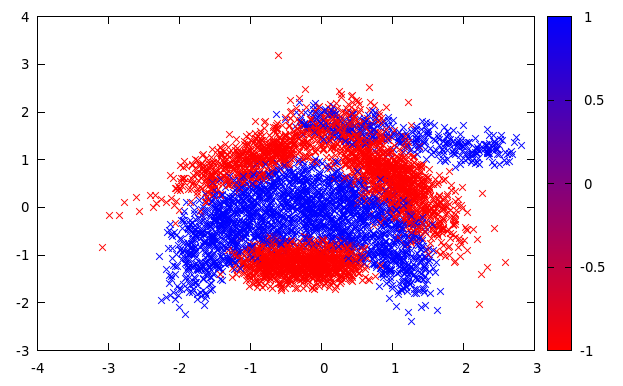
\includegraphics[scale=0.3]{banana.png}}
	\subfigure[CNN]{\label{fig:b}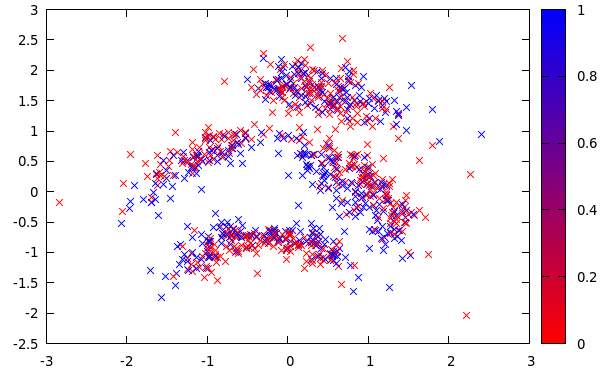
\includegraphics[scale=0.3]{CNN.png}}
	\subfigure[ENN]{\label{fig:c}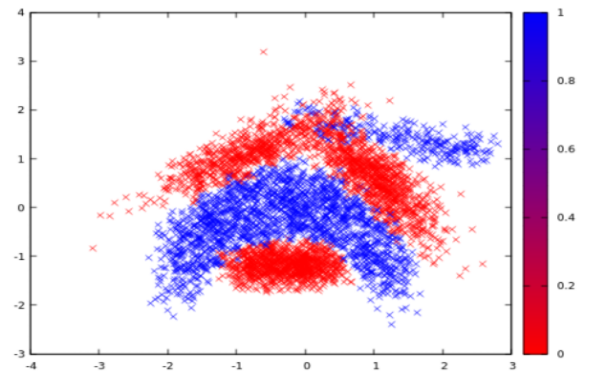
\includegraphics[scale=0.3]{ENN.png}}
	\subfigure[RSS]{\label{fig:d}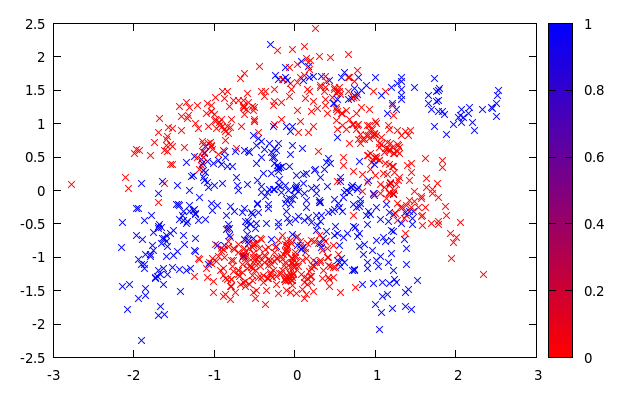
\includegraphics[scale=0.3]{RSS.png}}

\caption{Selección de instancias de las heurísticas}
\label{heu}
\end{figure}


Para presentar los resultados, se usan tablas que contienen los promedios en \emph{accuracy}, \emph{kappa}, reducción y tiempo de cómputo medido en segundos para cada heurística. \emph{Accuracy y kappa} se miden sobre los conjuntos de entrenamiento y prueba, la reducción mide el porcentaje de instancias eliminadas del conjunto original; a mayor \emph{accuracy, kappa} y reducción mejor es la heurística. Las pruebas fueron realizadas para los conjuntos pequeños, medianos y grandes por separado. Además, para determinar cuál si una metaheurística es mejor que otra se utiliza una prueba de \emph{Wilcoxon} de rango con signo con un nivel de significacia de 1\%, donde la hipótesis nula implica que las medidas son estadísticamente iguales y la hipótesis alternativa indica que existe una diferencia real entre las medidas.

Los experimentos fueron hechos con un procesador Intel(R) Core(TM) i5-3470 CPU @ 3.20GHz, 4 procesadores y 4GB de memoria RAM. Se utilizó C++ como lenguaje de programación y se compiló con GCC v.7.3.0.

\section{Resultados}

\subsection{Heurísticas}

En esta sección se busca estudiar el comportamiento de CNN, ENN y RSS al ser usados para resolver el problema de selección de prototipos sobre conjuntos de datos de tamaño pequeño, mediano y grande. De los resultados obtenidos, se espera determinar cuál heurística presenta los mejores niveles de \emph{accuracy, kappa} y reducción; además se busca evaluar el tiempo de cómputo de cada heurística.


\begin{table}[h!]
\centering
\begin{tabular}{l c c c c c c}
\hline
\multirow{2}{*}{\textsc{Algoritmo}}
	& \multicolumn{2}{c}{\textsc{Accuracy}}
	& \multicolumn{2}{c}{\textsc{Kappa}}
	& \textsc{Reducción}
	& \textsc{Tiempo (seg)} \\
	& Training & Test
	& Training & Test \\ 
\hline
\hline

Pequeños\\
CNN & 0.9093 & 0.7447 & 0.8396 & 0.5404 & 0.7380 & 0.1351 \\
ENN & 0.8563 & 0.7924 & 0.7319 & 0.6120 & 0.2591 & 0.1815 \\
RSS & 0.8363 & 0.7499 & 0.6997 & 0.5426 & 0.7308 & 0.1231 \\

\hline

Medianos\\
CNN & 0.8944 & 0.7823 & 0.7611 & 0.5613 & 0.7437 & 0.7108 \\
ENN & 0.8402 & 0.7999 & 0.6842 & 0.5863 & 0.2861 & 1.2668 \\
RSS & 0.8619 & 0.7922 & 0.6822 & 0.5524 & 0.6477 & 0.9201 \\

\hline

Grandes\\
CNN & 0.8818 & 0.8158 & 0.7396 & 0.5587 & 0.8183 & 3.2853 \\
ENN & 0.9355 & 0.8895 & 0.7938 & 0.6463 & 0.1495 & 6.1658 \\
RSS & 0.9176 & 0.8731 & 0.7411 & 0.6007 & 0.7236 & 10.7264 \\


\hline
\end{tabular}
\caption{Promedios de heurísticas}
\label{heu}
\end{table}

Al estudiar los resultados presentes en la tabla \ref{heu}, se puede destacar:

\begin{itemize}

\item ENN es la heurística que presenta los mejores niveles de \emph{accuracy y kappa} en la validación (\emph{test}) para los conjuntos de los tres tamaños. Esto se debe a que ENN es la heurística que menos instancias elimina y por lo tanto el conjunto $S$ resultante se asemeja bastante al conjunto original, lo cual le permite mantener buenos niveles de representación.

\item CNN es la heurística que tiene los mayores niveles de reducción. Además, se puede observar que CNN presenta sobre-entrenamiento (\emph{overfitting}) tanto en \emph{accuracy} como en \emph{kappa}; lo cual se hace evidente por la marcada diferencia entre los valores obtenidos en los conjuntos de entrenamiento (\emph{training}) y los valores obtenidos en los conjuntos de validación (\emph{test}), donde 29.92\% es la diferencia más grande presente en el \emph{kappa} para los conjuntos pequeños. Tanto los buenos niveles de reducción como el sobre-entrenamiento suceden porque CNN elige sólo las instancias limítrofes entre clases para construir el conjunto $S$, donde elimina la mayoría de las instancias, que se concentran en la parte interna del espacio y por lo tanto, pierde parte del nivel de representación del conjunto original.

\item RSS presenta niveles similares de \emph{accuracy y kappa} a los vistos para CNN en los conjuntos pequeños y medianos, y niveles superiores en los conjuntos grandes. Por otra parte, presenta niveles superiores de reducción a los vistos para ENN. RSS representa un balance entre \emph{accuracy, kappa} y reducción producto de una selección mixta de instancias internas y limítrofes.


\end{itemize}

En conclusión, si se busca mantener los mejores niveles de \emph{accuracy y kappa} sin importar los niveles de reducción, ENN es la opción indicada porque mantiene casi todo el conjunto original intacto. En cambio, si se busca la máxima reducción posible, al dejar en segundo plano el \emph{accuracy y kappa}, CNN es la opción sugerida. Sin embargo, para mantener un equilibrio entre las tres mediciones, RSS es la mejor opción.

Al evaluar los tiempos de cómputo presentes en la tabla \ref{heu} se pueden observar los siguientes detalles:

\begin{itemize}

\item CNN es la heurística más rápida y es la que mejor escala a conjuntos de tamaño grande. Su rapidez sucede porque el algoritmo empieza con un conjunto vacío y agrega instancias conforme a los errores de clasificación que encuentra en cada iteración, deteniéndose cuando logra pasar una iteración sin errores. Este esquema le permite a CNN terminar rápidamente en la mayoría de los casos, independientemente del tamaño del conjunto a reducir, porque el conjunto de referencia con el que se hacen las clasificaciones siempre se mantiene pequeño. Se debe acotar que CNN, siendo un algoritmo con componentes estocásticos, puede tardar más del tiempo esperado en dar una solución porque, dependiendo del orden de presentación de las instancias, CNN puede llegar a necesitar varios iteraciones sobre el conjunto original para terminar; para casos patológicos, CNN puede llegar a tener una complejidad de $O(n^2*log(n))$, cuando el tiempo esperado normalmente es de $O(n*log(n))$.

\item ENN presenta los segundos mejores tiempos entre las tres heurísticas. EL tiempo adicional que le toma a ENN devolver una solución en comparación a CNN se debe a que ENN empieza con el conjunto original en su totalidad y en cada iteración elimina una instancia que no concuerda con la clase de su vecino más cercano. Sin embargo, como ENN sólo tiene que revisar cada instancia una sola vez, puede terminar en un buen tiempo inclusive con los conjuntos grandes. ENN tiene una complejidad de $O(n*log(n))$  

\item RSS es la heurística que presenta el crecimiento en tiempo de cómputo más pronunciado, ya que se requiere para terminar con un conjunto grande 10 veces más el tiempo requerido por un conjunto mediano. Este detalle de escalabilidad se debe a que RSS primero debe ordenar todas las instancias según la distancia a sus enemigos más cercanos, lo cual domina el tiempo del algoritmo y asintóticamente lo vuelve $O(n*log(n))$. Sin embargo, hay que tomar en cuenta que los tiempos son buenos para los conjuntos grandes, ya que regresa un resultado en aproximadamente 10 segundos; tiempo que es significativamente menor a lo requerido por los algoritmos evolutivos, como se verá en las secciones siguientes.

\end{itemize}

Una vez considerado los tiempos, se concluye que las tres heurísticas son una opción viable para reducir los datos dependiendo de las prioridades del usuario como se explicó anteriormente. Inclusive, los problemas de escalamiento presentes en RSS son mitigados con el uso de la estratificación, por lo que es la mejor opción si el usuario busca un balance entre \emph{accuracy, kappa} y reducción.



\subsection{Metaheurísticas}

En esta sección se estudia el comportamiento de GGA, SSGA, MA y CHC, con población inicial aleatoria, al resolver el problema de selección de instancias sobre conjuntos pequeños, medianos y grandes. El objetivo es determinar cuál algoritmo presenta los mejores niveles de \emph{accuracy, kappa} y reducción para los conjuntos de los distintos tamaños. Además, se estudia el tiempo que requiere cada algoritmo en dar una solución, con lo que se busca evaluar si hay una buena relación entre tiempo y calidad de los resultados.


\begin{table}[h!]
\centering
\begin{tabular}{l c c c c c c}
\hline
\multirow{2}{*}{\textsc{Algoritmo}}
	& \multicolumn{2}{c}{\textsc{Accuracy}}
	& \multicolumn{2}{c}{\textsc{Kappa}}
	& \textsc{Reducción}
	& \textsc{Tiempo (seg)} \\
	& Training & Test
	& Training & Test \\ 
\hline
\hline

Pequeños\\
GGA  & 0.8312 & 0.7525 & 0.7017 & 0.5557 & 0.5532 & 12.8250 \\
SSGA & 0.8654 & 0.7716 & 0.7635 & 0.5917 & 0.8432 & 0.6655 \\
MA   & 0.8570 & 0.7918 & 0.7440 & 0.6216 & 0.9561 & 4.1047 \\
CHC & 0.8446 & 0.7843 & 0.7172 & 0.6084 & 0.9466 & 0.5266 \\

\hline

Medianos\\
GGA  & 0.8702 & 0.7982 & 0.7375 & 0.5812 & 0.5641 & 110.0812 \\
SSGA & 0.8431 & 0.8029 & 0.6676 & 0.5871 & 0.8392 & 3.5589 \\
MA   & 0.8057 & 0.7908 & 0.5825 & 0.5564 & 0.9624 & 73.3461 \\
CHC  & 0.8313 & 0.8115 & 0.6347 & 0.5986 & 0.9455 & 2.8843 \\

\hline
Grandes\\
GGA  & 0.9316 & 0.8644 & 0.7994 & 0.6014 & 0.5050 & 672.0273 \\
SSGA & 0.8911 & 0.8743 & 0.6953 & 0.6201 & 0.8056 & 27.6637 \\
MA   & 0.8904 & 0.8999 & 0.6499 & 0.6510 & 0.9973 & 256.1432 \\
CHC  & 0.8961 & 0.8934 & 0.6614 & 0.6506 & 0.9615 & 16.8665 \\

\hline
\end{tabular}
\caption{Promedios de las metaheurísticas}
\label{meta}
\end{table}

Al estudiar los resultados obtenidos en la tabla \ref{meta}, se puede destacar los siguientes puntos sobre \emph{accuracy y kappa}:

\begin{itemize}

\item CHC y MA presentan los mejores niveles de \emph{accuracy y kappa} para los conjuntos de validación pequeños y grandes. Esto se atribuye a los mecanismos internos que tiene cada algoritmo para hacer la mejor selección de instancias posible. MA tiene su función de optimización que elimina todas las instancias posibles sin perjudicar el \emph{accuracy}, lo que permite mejorar al máximo cada cromosoma de la población; mientras que CHC tiene su mecanismo de prevención de incesto para crear cromosomas lo más distinto posible de los padres, además de tener la capacidad de reiniciar su población, tomando como base el mejor cromosoma encontrado, para evitar la convergencia prematura de la misma.

\item SSGA presenta niveles similares de \emph{accuracy y kappa} que GGA para los conjuntos de validación de pequeños y grandes. Ambos algotirmos presentan niveles inferiores que CHC y MA producto de una selección de instancias menos informada que estos últimos. La única manera estable que tienen GGA y SSGA para obtener mejores resultados es a través de la operación de cruce, mientras que MA y CHC cuentan con las herramientas antes mencionadas.

\item Para los conjuntos medianos, las cuatro metaheurísticas obtuvieron un nivel de \emph{accuracy} similar. Mientras que MA obtuvo un nivel de \emph{kappa} inferior a los otros tres métodos. Este comportamiento de las metaheurísticas frente a los conjuntos medianos se atribuye directamente a la topología (cómo se encuentran organizadas las soluciones en el espacio) de los conjuntos de datos utilizados para realizar las pruebas; lo que deja en evidencia la influencia que tiene el conjunto de datos sobre el comportamiento de los algoritmos.

\end{itemize}

En relación a la reducción se puede observar:

\begin{itemize}

\item MA es la metaheurística que presenta los mayores niveles de reducción. Este hecho se vuelve a atribuir a el proceso de optimización interna, ya que es un proceso de intensificación en el cual se refina un cromosoma a uno con la mínima cardinalidad posible sin perder \emph{accuracy}.

\item CHC alcanza buenos niveles de reducción, gracias a la selección totalmente elitista de los cromosomas que siempre realiza en cada iteración (sólo se preservan los mejores cromosomas y es a partir del mejor que se reinicia la población). Como uno de los componentes que comforma la función objetivo es la tasa de reducción, CHC naturalmente favorece aquellas soluciones con pocas instancias que puedan mantener buenos valores de \emph{accuracy y kappa}.

\item GGA presenta los niveles más bajos de reducción, esto ocurre porque no posee mecanismos de preservación elitistas como en el caso de CHC. GGA se caracteriza por perder toda la información acumulada en una generación de cromosomas (excepto el mejor), eliminando cromosomas que podrían generar mejores soluciones si se les diera más oportunidades de ser cruzados. Además, GGA carece de procesos de intensificación como los tiene MA, lo cual vuelve más difícil la eliminación de instancias.

\item SSGA presenta mejores niveles de reducción a los obtenidos por GGA porque usa un método simple de elitismo, en el cual en cada iteración sólo se generan dos cromosomas nuevos (a diferencia de una población entera) y éstos sólo suplantan a sus padres si son mejores. Este mecanismo permite que la cantidad de instancias disminuya paulatinamente hasta llegar a la convergencia de la población.

\end{itemize}

En relación a los tiempos de cómputo se puede destacar:

\begin{itemize}

\item CHC es la metaheurística que necesita menos tiempo en dar una solución. Esto se debe a su operador de cruce, el cual tarda tiempo lineal ($O(n)$) y permite hacer una búsqueda diversificada del espacio de soluciones de manera inteligente, ya que, a partir de unos cromosomas seleccionados de manera elitista, genera nuevos cromosomas que son lo más distinto posible, mientras mantiene cualidades (las cuales se esperan que sean buenas) de sus padres. Estos detalles hacen posible la obtención de buenos resultados rápidamente.

\item SSGA es otra metaheurística que no necesita mucho tiempo en dar una solución. La razón de esto es parecida a la de CHC, ya que el operador de cruce toma tiempo lineal y en cada iteración sólo se generan 2 cromosomas, lo cual lleva al algoritmo a terminar rápidamente.

\item MA tarda significativamente más en regresar una solución en comparación a CHC y SSGA. Para los conjuntos pequeños, MA tarda 7 veces más que CHC; para los conjuntos medianos, MA tarda 25 veces más que CHC y para los conjuntos grandes, MA tarda 15 veces más. Esta diferencia en tiempo se debe al proceso de optimización interna que usa MA en cada iteración, el cual es $O(n^2)$.

\item GGA es la metaheurística que más tarda en dar una solución. Esto se debe a que en cada iteración, GGA debe generar una población de cromosomas nuevo, a diferencia de SSGA que sólo genera dos cromosomas.

\item CHC y SSGA son las metaheurísticas que mejor escalan a los conjuntos grandes, ya que mantienen los tiempos de ejecución por debajo de 30 segundos, teniendo valores no muy alejados de los tiempos obtenidos por las heurísticas. Por otra parte, GGA y MA sobrepasan los 200 segundos en tiempo de cómputo, lo cual es 20 veces más lo que tardan CNN, ENN y RSS. Sin embargo, hay que tomar en cuenta que la estratificación ayuda a reducir significativamente los tiempos de cómputo de las cuatro metaheurísticas, al punto de que es factible aplicar los cuatro algoritmos a los conjuntos grandes; ya que en trabajos como los realizados por \emph{Cano, J. et al.} en \cite{garcia2008memetic} y \cite{garcia2012prototype} no se pudo probar estos algoritmos sin el uso de estratificación por la gran cantidad de tiempo que tomarían en devolver una respuesta.

\end{itemize}


\begin{figure}[h!]

	\centering
	\subfigure[\emph{Accuracy} + reducción]{\label{fig:a}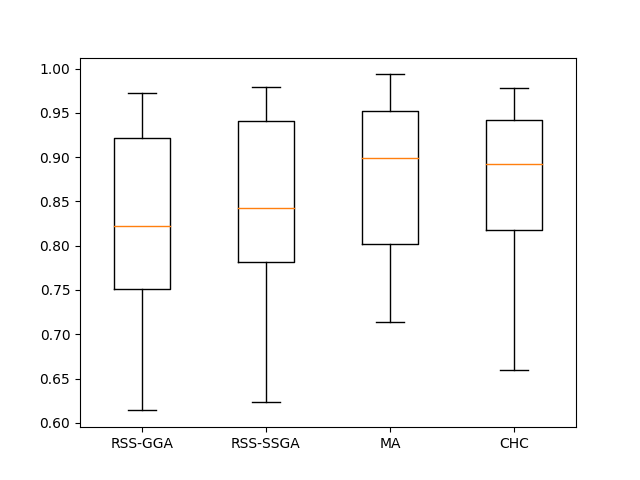
\includegraphics[scale=0.4]{acc_small.png}}
	\subfigure[\emph{kappa} + reducción]{\label{fig:b}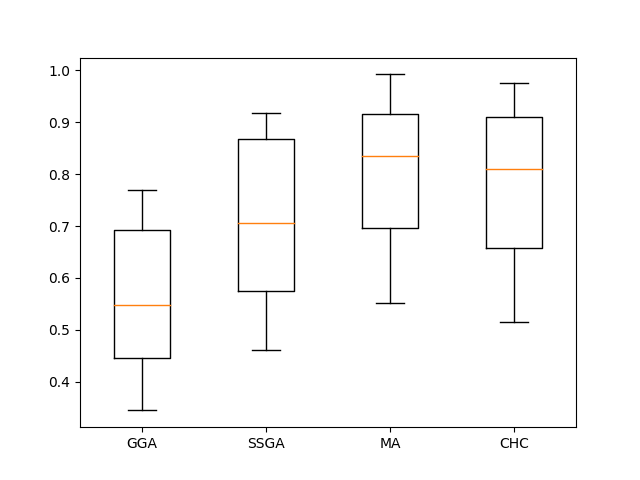
\includegraphics[scale=0.4]{kappa_small.png}}

\caption{Boxplots de las metaheurísticas para los conjuntos pequeños}
\label{small-heuristics}
\end{figure}

\begin{figure}[h!]

	\centering
	\subfigure[\emph{Accuracy} + reducción]{\label{fig:a}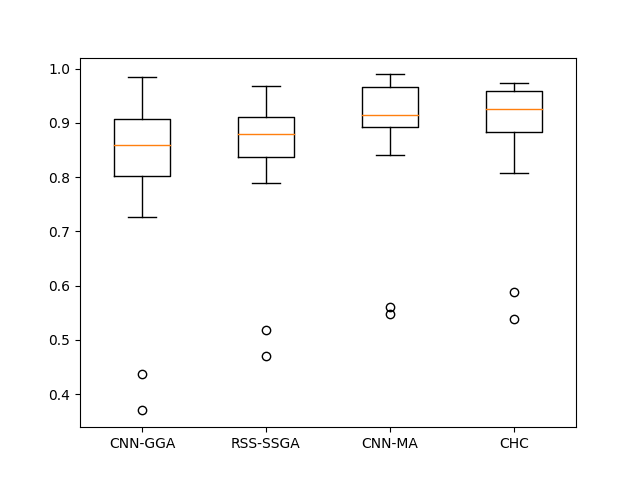
\includegraphics[scale=0.4]{acc_medium.png}}
	\subfigure[\emph{kappa} + reducción]{\label{fig:b}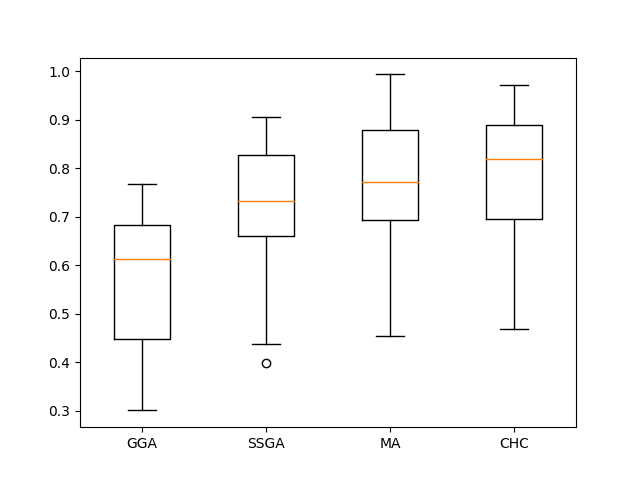
\includegraphics[scale=0.4]{kappa_medium.png}}

\caption{Boxplots de las metaheurísticas para los conjuntos medianos}
\label{medium-heuristics}
\end{figure}

Las figuras \ref{small-heuristics} y \ref{medium-heuristics} muestran que cuando se toma en cuenta la combinación lineal de \emph{accuracy} + reducción y \emph{kappa} + reducción, MA y CHC presentan los niveles más elevados. Cabe destacar que las tablas \ref{wilcox-meta-peq} y \ref{wilcox-meta-med} del Apéndice A muestran que los p-valores de la comparación entre MA y CHC para los conjuntos pequeños son 6.934e-02 para \emph{accuracy} + reducción y  7.80e-02 para \emph{kappa} + reducción. Por su parte, para los conjuntos medianos se tiene 6.009e-01 y 7.172e-01 respectivamente; lo cual implica que MA y CHC son estadísticamente similares. 

De acuerdo a la información presentada anteriormente, se puede concluir que CHC es la mejor metaheurística para resolver el problema de selección de prototipos para los conjuntos pequeños, medianos y grandes. Ya que, junto a MA presenta los valores más elevados de \emph{accuracy, kappa} y reducción, con la peculiaridad de que es la metaheurística que menos tiempo tarda en regresar un resultado. Lo cual lo hace el candidato ideal al momento de aumentar el tamaño de los conjuntos de datos.  



\subsection{Variaciones de las metaheurísticas}

Después del proceso anterior, el paso inmediato a seguir es la combinación de las heurísticas con las metaheurísticas. La idea es evaluar las variaciones de cada metaheurística por separado, de tal manera de que se se identifique cuál heurística beneficia más a la metaheurística. La notación en la columna de ``\textsc{Algoritmo}'' indica primero qué heurística se usó para inicializar la población y le sigue la metaheurística usada; un ejemplo es CNN-GGA, que indica que CNN es la heurística usada para inicializar la población de la metaheurística GGA. Para el caso de usar una población incial aleatoria, se coloca simplemente el nombre de la metaheurística. La mejor variación de cada metaheurística se encuentra sombreada.


\subsubsection{Conjuntos pequeños}

En esta sección se estudia el comportamiento de las variaciones de GGA, SSGA, MA y CHC al resolver el problema de selección de instancias sobre conjuntos pequeños. El objetivo es determinar cuál algoritmo presenta los mejores niveles de \emph{accuracy, kappa} y reducción. Además, se estudia el tiempo que requiere cada algoritmo en dar una solución, con lo que se busca evaluar si hay una buena relación entre tiempo y calidad de los resultados.


\begin{table}[h!]
\centering
\begin{tabular}{l c c c c c c}
\hline
\multirow{2}{*}{\textsc{Algoritmo}}
	& \multicolumn{2}{c}{\textsc{Accuracy}}
	& \multicolumn{2}{c}{\textsc{Kappa}}
	& \textsc{Reducción}
	& \textsc{Tiempo (seg)} \\
	& Training & Test
	& Training & Test \\ 
\hline
\hline

\textbf{GGA}         & \textbf{0.8312} & \textbf{0.7525} & \textbf{0.7017} & \textbf{0.5557} & \textbf{0.5532} & \textbf{12.8250} \\
CNN-GGA     & 0.5736 & 0.4911 & 0.3525 & 0.2151 & 0.7491 & 33.4671 \\
ENN-GGA     & 0.8533 & 0.7891 & 0.7327 & 0.6093 & 0.2611 & 14.6024 \\
RSS-GGA     & 0.6626 & 0.6177 & 0.4044 & 0.3263 & 0.7717 & 21.5376 \\
CNN-RSS-GGA & 0.7883 & 0.6809 & 0.6353 & 0.4472 & 0.6221 & 43.1002 \\
ENN-RSS-GGA & 0.8973 & 0.7872 & 0.8182 & 0.6063 & 0.1994 & 36.5439 \\

\hline

SSGA & 0.8654 & 0.7716 & 0.7635 & 0.5917 & 0.8432 & 0.6655 \\
CNN-SSGA & 0.8791 & 0.7695 & 0.7840 & 0.5815 & 0.8425 & 1.2187 \\
ENN-SSGA & 0.8733 & 0.7919 & 0.7683 & 0.6112 & 0.7823 & 0.8601 \\
\textbf{RSS-SSGA} & \textbf{0.8581} & \textbf{0.7726} & \textbf{0.7460} & \textbf{0.5905} & \textbf{0.8958} &\textbf{1.0116} \\
CNN-RSS-SSGA & 0.8808 & 0.7742 & 0.7884 & 0.5974 & 0.8373 & 1.9109 \\
EEN-RSS-SSGA & 0.8843 & 0.7890 & 0.7904 & 0.6134 & 0.7586 & 1.6563 \\

\hline

\textbf{MA}   & \textbf{0.8570} & \textbf{0.7918} & \textbf{0.7440} & \textbf{0.6216} & \textbf{0.9561} & \textbf{4.1047} \\
CNN-MA & 0.8653 & 0.7987 & 0.7519 & 0.6307 & 0.9486 & 5.9638 \\
ENN-MA & 0.8666 & 0.7930 & 0.7576 & 0.6215 & 0.9534 & 4.2491 \\
RSS-MA & 0.8446 & 0.7795 & 0.7137 & 0.5903 & 0.9630 & 4.6391 \\
CNN-RSS-MA  & 0.8639 & 0.7848 & 0.7538 & 0.6090 & 0.9507 & 8.9884 \\
ENN-RSS-MA & 0.8736 & 0.7942 & 0.7716 & 0.6268 & 0.9474 & 8.3942 \\

\hline

\textbf{CHC} & \textbf{0.8446} & \textbf{0.7843} & \textbf{0.7172} & \textbf{0.6084} & \textbf{0.9466} & \textbf{0.5266} \\
CNN-CHC & 0.8495 & 0.7812 & 0.7269 & 0.6027 & 0.9385 & 0.7891 \\
ENN-CHC & 0.8429 & 0.7863 & 0.7179 & 0.6132 & 0.9424 & 0.7445 \\
RSS-CHC & 0.8383 & 0.7779 & 0.6963 & 0.5836 & 0.9546 & 0.7137 \\
CNN-RSS-CHC  & 0.8442 & 0.7794 & 0.7099 & 0.5864 & 0.9437 & 1.1144 \\
ENN-RSS-CHC & 0.8484 & 0.7846 & 0.7224 & 0.6030 & 0.9333 & 1.0723 \\

\hline
\end{tabular}
\caption{Promedios de las distintas variaciones de cada metaheurística para los conjuntos pequeños}
\label{peq-all}
\end{table}

Al estudiar los resultados obtenidos en la tabla \ref{peq-all}, se pueden destacar los siguientes aspectos observados de las variaciones de GGA:

\begin{itemize}

\item GGA, ENN-GGA y ENN-RSS-GGA presentan los mejores niveles de \emph{accuracy y kappa}. Esto se debe a que son las variantes que preservan la mayor cantidad de instancias y por lo tanto el resultado mantiene un buen nivel de representación del conjunto original.

\item CNN-GGA presenta los niveles más bajos de \emph{accuracy}. Esto sucede porque la población inicial es bastante reducida y concentrada en las fronteras, debido a CNN, y GGA no posee los mecanismos para diversificar la población en búsqueda de mejores soluciones.

\item CNN-GGA y RSS-GGA presentan los niveles más bajos de \emph{kappa}, lo cual significa que los dos algoritmos generan conjuntos que incluyen principalmente elementos de la clase mayoritaria, dejando pocos representantes de las clases minoritarias que no ayudan a la correcta clasificación de las mismas. Estos valores por debajo del 35\% implican que entre los conjuntos pequeños hay conjuntos que están sesgados hacia una o más clases y los conjuntos construidos por CNN-GGA y RSS-GGA no logran representar correctamente las clases minoritarias.

\item RSS-GGA presenta los mejores niveles de reducción. Esto ocurre porque la selección mixta de instancias que hace RSS le permite a GGA tener una búsqueda diversificada por el espacio de soluciones, lo que facilita la obtención de resultados con menos instancias.

\item CNN-GGA también presenta buenos niveles de reducción porque CNN realiza casi toda la selección de instancias desde el principio.

\item ENN-GGA y ENN-RSS-GGA presentan las tasas más bajas de reducción. Esto ocurre porque ENN naturalmente deja la mayor cantidad de instancias y GGA carece de los medios para realizar una reducción significativa de un conjunto densamente poblado.

\item ENN-GGA y RSS-GGA son las variaciones, excluyendo a GGA, que menos tiempo toman en dar un resultado porque tanto ENN como RSS tienen una complejidad de $O(n*log(n))$ los cuales les permite devolver una respuesta rápidamente.

\item CNN-GGA tarda más que ENN-GGA y que RSS-GGA por una combinación de factores que incluyen: los componentes estocásticos de CNN, que pueden ocasionar una elevada cantidad de iteraciones hasta converger a un conjunto; y la probabilidad de cruce elegida para GGA, la cual es de 48.37\%, lo trae como consecuencia que pasen muchas iteraciones intentando cruzar cromosomas para formar todos los elementos de cada generación. Cabe destacar que el promedio de tiempo de cómputo de CNN-GGA se ve afectado por dos casos atípicos: \emph{Banknote} y \emph{Winsconsin} para los cuales se reportan 280.39 segundos y 272.64 segundos (véase tabla \ref{res-peq-cnn-gga} en el apéndice B) para que el algoritmo culmine.

\end{itemize}

De las observaciones anteriores se puede concluir que GGA con población inicial aleatoria es la mejor variación de GGA; esto se debe a que presenta el mejor balance entre \emph{accuracy, kappa} y reducción, además de que es la variente más rápida. El uso de heurísticas en este caso, no representa una mejoría significativa por el cual se justifique el costo adicional en tiempo que conlleva el uso de las heurísticas; las mismas introducen desequilibrios al enofarse únicamente en \emph{accuracy y kappa} (como el caso de ENN-GGA) o en reducción (como el caso de CNN).

Al pasar a los resultados obtenidos para las variaciones de SSGA, se puede observar:

\begin{itemize}

\item ENN-SSGA y ENN-RSS-SSGA presentan los mejores valores para \emph{accuracy y kappa} producto de usar un conjunto inicial con la mayoría de las instancias del conjunto original.

\item RSS-SSGA presenta la tasa de reducción más alta, gracias a la selección de instancias realizada por RSS, la cual introduce variedad en la búsqueda de SSGA.

\item La diferencia entre la tasa más alta y la más baja de reducción es de 13.72\%, siendo la tasa más baja la de ENN-RSS-SSGA con 75.86\%. Este resultado muestra que SSGA puede conseguir buenas tasas de reducción inclusive con un conjunto inicial muy parecido al conjunto original en cardinalidad.

\item Los mejores tiempos entre las variantes que usan heurísticas son los obtenidos por ENN-SSGA y RSS-SSGA, las razones son las mismas que las dadas para las variaciones de GGA. 

\end{itemize}

De las consideraciones anteriores, se puede concluir que RSS-SSGA es la mejor variación de SSGA, ya que presenta la mayor tasa de reducción, estando 5.26\% por encima de SSGA con población inicial aleatoria, y mantiene buenos niveles de \emph{accuracy y kappa}, razones que justifican el tiempo adicional de cómputo, que cabe destacar está por debajo de los dos segundos, lo que lo posiciona entre las metaheurísticas más rápidas.

Al evaluar los resultados obtenidos por las variaciones de MA, se observa:

\begin{itemize}

\item Todas las variaciones presentan valores similares de \emph{accuracy y kappa}. El mayor \emph{accuracy}, obtenido por ENN-RSS-MA, sólo está 0.24\% por encima del \emph{accuracy} obtenido por MA con población inicial aleatoria. A su vez, el \emph{kappa} obtenido por ENN-RSS-MA sólo está 0.52\% por encima del obtenido por MA. 

\item Todas las variaciones presentan tasas de reducción similares. RSS-MA, la variación que presenta la tasa de reducción más alta, está sólo 6.9e-03\% por encima de MA. 

\end{itemize}

Al revisar los resultados obtenidos por las variaciones de CHC, se observa:

\begin{itemize}

\item Todas las variaciones presentan valores similares de \emph{accuracy y kappa}. El mayor \emph{accuracy}, obtenido por ENN-CHC, sólo está 0.2\% por encima de CHC con población inicial aleatoria. Por su parte, el \emph{kappa} obtenido por ENN-CHC es sólo 0.48\% mayor que el obtenido por CHC.

\item Todas las variaciones obtuvieron tasas de reducción similares. RSS-CHC, la variación que presenta la tasa de reducción más alta, está sólo 0.8\% por encima de CHC.

\end{itemize}

De las observaciones anteriores se concluye que MA y CHC son metaheurísticas capaces de obtener resultados consistentes independientemente de la población inicial que utilicen. Por lo tanto el uso de heurísticas no conlleva a un beneficio real y sólo aumenta el tiempo de cómputo, razón por la cual MA y CHC con población incial aleatoria son las mejores varientes de sus respectivas metaheurísticas.


Las figuras \ref{small-accu-all} y \ref{small-kap-all} muestran \emph{boxplots} de todas las variaciones de metaheurísticas para los conjuntos pequeños, de izquierda a derecha los \emph{boxplots} representan las siguientes variaciones: '1':GGA, '2':CNN-GGA, '3':ENN-GGA, '4':RSS-GGA, '5':CNN-RSS-GGA, '6':ENN-RSS-GGA, '7':SSGA, '8':CNN-SSGA, '9':ENN-SSGA, '10':RSS-SSGA, '11':CNN-RSS-SSGA, '12':ENN-RSS-SSGA, '13':MA, '14':CNN-MA, '15':ENN-MA, '16':RSS-MA, '17':CNN-RSS-MA, '18':ENN-RSS-MA, '19':CHC, '20':CNN-CHC, '21':ENN-CHC, '22':RSS-CHC, '23':CNN-RSS-CHC y '24':ENN-RSS-CHC.

\begin{figure}[h!]

	\centering
	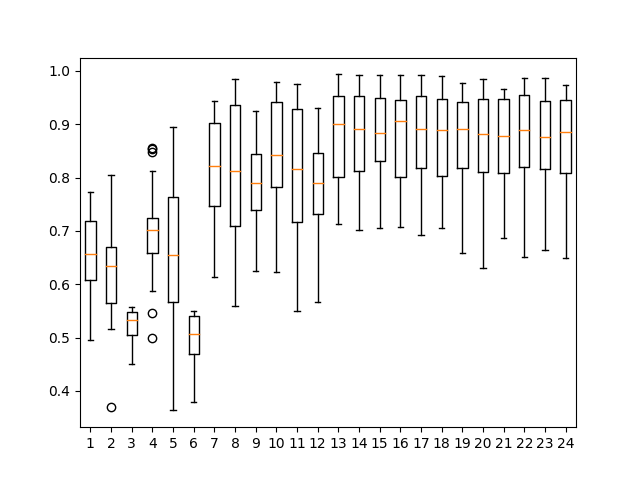
\includegraphics[scale=0.8]{acc_small_all.png}

\caption{\emph{Accuracy} + reducción de las variaciones de las metaheurísticas para los conjuntos pequeños}
\label{small-accu-all}
\end{figure}


\begin{figure}[h!]

	\centering
	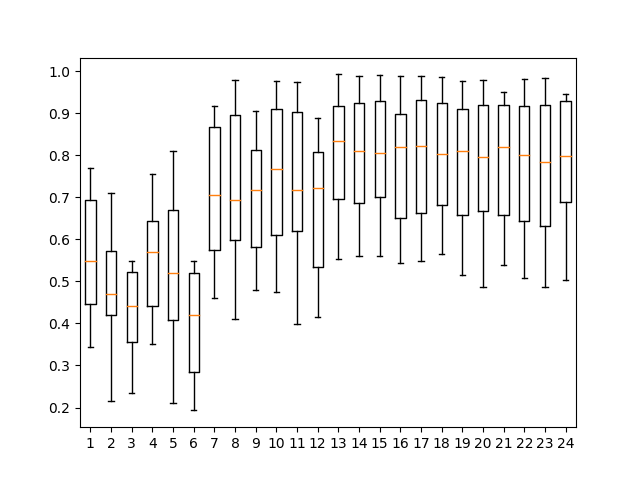
\includegraphics[scale=0.8]{kappa_small_all.png}

\caption{\emph{Kappa} + reducción de las variaciones de las metaheurísticas para los conjuntos pequeños}
\label{small-kap-all}
\end{figure}

Los \emph{boxplots} que van desde el número 13 hasta el 18 confirman que todas las variantes de MA presentan valores similares. Esto también sucede con CHC al ver los \emph{boxpĺots} que van desde el 19 hasta el 24. Los p-valores de las tablas \ref{wilcox-MA-peq} y \ref{wilcox-CHC-peq} en el anexo A muestran que todas las variantes son estadísticamente similares en \emph{accuracy} + reducción y \emph{kappa} + reducción.

De las figuras \ref{small-accu-all} y \ref{small-kap-all} también se puede apreciar que las variantes de MA y las de CHC presentan valores similares. Los resultados de la prueba \emph{Wilcoxon} (ver tabla \ref{wilcox-best-peq} en el anexo A) para MA y CHC muestran p-valores iguales a 6.934e-02 para \emph{accuracy} + reducción y 7.800e-02 para \emph{kappa} + reducción, lo que implica que ambos algoritmos son estadísticamente similares.

Como la diferencia entre MA y CHC es el tiempo de cómputo, se tiene que CHC con población inicial aleatoria presenta los tiempos más cortos y por lo tanto es la mejor metaheurística para resolver el problema de selección de prototipos sobre conjuntos pequeños.


\subsubsection{Conjuntos medianos}

En esta sección se estudia el comportamiento de las variaciones de GGA, SSGA, MA y CHC al resolver el problema de selección de instancias sobre conjuntos medianos. El objetivo es determinar cuál algoritmo presenta los mejores niveles de \emph{accuracy, kappa} y reducción. Además, se estudia el tiempo que requiere cada algoritmo en dar una solución, con lo que se busca evaluar si hay una buena relación entre tiempo y calidad de los resultados.


\begin{table}[h!]
\centering
\begin{tabular}{l c c c c c c}
\hline
\multirow{2}{*}{\textsc{Algoritmo}}
	& \multicolumn{2}{c}{\textsc{Accuracy}}
	& \multicolumn{2}{c}{\textsc{Kappa}}
	& \textsc{Reducción}
	& \textsc{Tiempo (seg)} \\
	& Training & Test
	& Training & Test \\ 
\hline
\hline

\textbf{GGA}         & \textbf{0.8702} & \textbf{0.7982} & \textbf{0.7375} & \textbf{0.5812} & \textbf{0.5641} & \textbf{110.0812} \\
CNN-GGA     & 0.7990 & 0.7051 & 0.5952 & 0.4426 & 0.7745 & 232.8342 \\
ENN-GGA     & 0.8475 & 0.8071 & 0.6949 & 0.5965 & 0.2862 & 125.8465 \\
RSS-GGA     & 0.8027 & 0.7520 & 0.5575 & 0.4547 & 0.6733 & 137.0381 \\
CNN-RSS-GGA & 0.8932 & 0.7890 & 0.7571 & 0.5516 & 0.5514 & 309.4603 \\
ENN-RSS-GGA & 0.9141 & 0.8155 & 0.8246 & 0.6168 & 0.1981 & 314.2968 \\

\hline

SSGA & 0.8431 & 0.8029 & 0.6676 & 0.5871 & 0.8392 & 3.5589 \\
CNN-SSGA & 0.8540 & 0.8007 & 0.6965 & 0.5923 & 0.8547 & 6.4410 \\
ENN-SSGA & 0.8200 & 0.8009 & 0.6324 & 0.5793 & 0.7459 & 5.6722 \\
\textbf{RSS-SSGA} & \textbf{0.8302} & \textbf{0.8045} & \textbf{0.6389} & \textbf{0.5854} & \textbf{0.8690} & \textbf{5.9946} \\
CNN-RSS-SSGA & 0.8586 & 0.8047 & 0.7043 & 0.5977 & 0.8121 & 10.5868 \\
ENN-RSS-SSGA & 0.8550 & 0.8078 & 0.7042 & 0.6004 & 0.7049 & 10.4293 \\

\hline

MA   & 0.8057 & 0.7908 & 0.5825 & 0.5564 & 0.9624 & 73.3461 \\
\textbf{CNN-MA} & \textbf{0.8116} & \textbf{0.8021} & \textbf{0.6000} & \textbf{0.5765} & \textbf{0.9572} & \textbf{57.3939} \\
ENN-MA & 0.7938 & 0.7925 & 0.5747 & 0.5608 & 0.9707 & 67.5310 \\
RSS-MA & 0.7924 & 0.7893 & 0.5611 & 0.5449 & 0.9671 & 69.5927 \\
CNN-RSS-MA & 0.8051 & 0.8015 & 0.5962 & 0.5808 & 0.9654 & 121.2220 \\
ENN-RSS-MA & 0.8070 & 0.7971 & 0.5886 & 0.5653 & 0.9633 & 112.0309 \\

\hline

\textbf{CHC} & \textbf{0.8313} & \textbf{0.8115} & \textbf{0.6347} & \textbf{0.5986} & \textbf{0.9455} & \textbf{2.8843} \\
CNN-CHC & 0.8303 & 0.8081 & 0.6337 & 0.5925 & 0.9352 & 4.6572 \\
ENN-CHC & 0.8107 & 0.8032 & 0.6084 & 0.5834 & 0.9356 & 5.0976 \\
RSS-CHC & 0.8151 & 0.8058 & 0.6074 & 0.5851 & 0.9535 & 4.7450 \\
CNN-RSS-CHC & 0.8276 & 0.8073 & 0.6280 & 0.5871 & 0.9319 & 6.7859 \\
ENN-RSS-CHC  & 0.8255 & 0.8074 & 0.6355 & 0.5944 & 0.9154 & 7.0284 \\


\hline
\end{tabular}
\caption{Promedios de las distintas variaciones de cada metaheurística para los conjuntos medianos}
\label{med-all}
\end{table}

Al estudiar los resultados obtenidos en la tabla \ref{med-all}, se pueden destacar los siguientes aspectos observados de las variaciones de GGA:

\begin{itemize}

\item GGA, ENN-GGA y ENN-RSS-GGA presentan los mejores niveles de \emph{accuracy y kappa}.

\item CNN-GGA presenta los niveles más bajos de \emph{accuracy}.

\item CNN-GGA y RSS-GGA presentan los niveles más bajos de \emph{kappa}. Al considerar que las otras variaciones obtienen un \emph{kappa} superior al 55\%, mientras que CNN-GGA y RSS-GGA obtienen valores por debajo del 46\%, se puede concluir que estas últimas tienen problemas para distinguir las clases minoritarias.

\item CNN-GGA presenta la tasa de reducción más alta con 77.45\%.

\item ENN-GGA y ENN-RSS-GGA presentan las tasas más bajas de reducción.

\item ENN-GGA y RSS-GGA son las variaciones, excluyendo a GGA, que menos tiempo toman en dar un resultado.

\end{itemize}

De las observaciones anteriores se puede concluir que GGA con población inicial aleatoria es la mejor variación de GGA; esto se debe a que presenta el mejor balance entre \emph{accuracy, kappa} y reducción, además de que es la variente más rápida. Cabe destacar CNN-GA porque presenta un \emph{accuracy} superior al 70\% a la vez que tiene la tasa de reducción más alta (21.04\% por encima de GGA); sin embargo, compromete los valores de \emph{kappa} (13.86\% por debajo de GGA) y tarda aproximadamente el doble de tiempo que GGA para dar una respuesta, razones que desfavorecen a CNN-GGA al momento de elegir una variante para resolver el problema de selección de prototipos.

Al pasar a los resultados obtenidos para las variaciones de SSGA, se puede observar:

\begin{itemize}

\item Todas las variaciones presentan niveles similares de \emph{accuracy}.

\item ENN-RSS-SSGA presenta el porcentaje más alto de \emph{kappa}, 1.33\% por encima de SSGA.

\item RSS-SSGA presenta la tasa de reducción más alta, 2.98\% por encima de SSGA.

\item Los mejores tiempos entre las variantes que usan heurísticas son los obtenidos por ENN-SSGA y RSS-SSGA. Ambas medidas se encuentran por debajo de los 7 segundos. 

\end{itemize}

Como los resultados entre las variaciones son muy similares, se necesita evaluar los p-valores de la prueba \emph{Wilcoxon}. En la tabla \ref{wilcox-SSGA-med} del apéndice A se puede apreciar que el p-valor de comparar RSS-SSGA con SSGA en \emph{accuracy} + reducción es de 7.013e-03, lo que implica que existe una diferencia estadística entre los dos algoritmos. Por lo tanto RSS-SSGA, que presenta la mayor tasa de reducción a la vez que mantiene buenos niveles de \emph{accuracy y kappa}, se puede considerar la mejor variación de SSGA.

Al evaluar los resultados obtenidos por las variaciones de MA, se observa:

\begin{itemize}

\item Todas las variaciones presentan valores similares de \emph{accuracy y kappa}.

\item Todas las variaciones presentan tasas de reducción similares.

\item CNN-MA es la variación que menos tarda en devolver un resultado entre todas, incluso tardando menos que CNN con población inicial aleatoria. Esto se debe a que con la población proporcionada por CNN se disminuyó el número de veces que MA utilizó el proceso de optimización interna.

\end{itemize}

Al revisar los resultados obtenidos por las variaciones de CHC, se observa:

\begin{itemize}

\item Todas las variaciones presentan valores similares de \emph{accuracy y kappa}.

\item CHC, CNN-CHC, ENN-CHC, RSS-CHC y CNN-RSS-CHC obtuvieron tasas de reducción similares. ENN-RSS-CHC, por su parte, obtuvo las tasas más bajas de reducción, estando 3.01\% por debajo de CHC. Esta diferencia es estadísticamente significativa al observar los resultados de los p-valores para reducción en la tabla \ref{wilcox-CHC-med} del anexo A.

\end{itemize}

De las observaciones anteriores se concluye que MA y CHC son metaheurísticas capaces de obtener resultados consistentes independientemente de la población inicial que utilicen. La decisión de cuales son las mejores variaciones depende del tiempo de cómputo: en el caso de MA, la mejor variación es CNN-MA; en el caso de CHC, CHC con población inicial aleatoria es la mejor.


Las figuras \ref{medium-accu-all} y \ref{medium-kap-all} muestran \emph{boxplots} de todas las variaciones de metaheurísticas para los conjuntos medianos, de izquierda a derecha los \emph{boxplots} representan las siguientes variaciones: '1':GGA, '2':CNN-GGA, '3':ENN-GGA, '4':RSS-GGA, '5':CNN-RSS-GGA, '6':ENN-RSS-GGA, '7':SSGA, '8':CNN-SSGA, '9':ENN-SSGA, '10':RSS-SSGA, '11':CNN-RSS-SSGA, '12':ENN-RSS-SSGA, '13':MA, '14':CNN-MA, '15':ENN-MA, '16':RSS-MA, '17':CNN-RSS-MA, '18':ENN-RSS-MA, '19':CHC, '20':CNN-CHC, '21':ENN-CHC, '22':RSS-CHC, '23':CNN-RSS-CHC y '24':ENN-RSS-CHC.

\begin{figure}[h!]

	\centering
	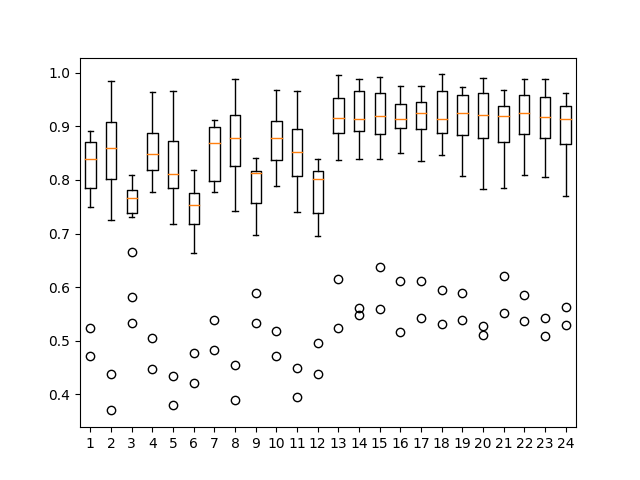
\includegraphics[scale=0.8]{acc_medium_all.png}

\caption{\emph{Accuracy} + reducción de las variaciones de las metaheurísticas para los conjuntos medianos}
\label{medium-accu-all}
\end{figure}


\begin{figure}[h!]

	\centering
	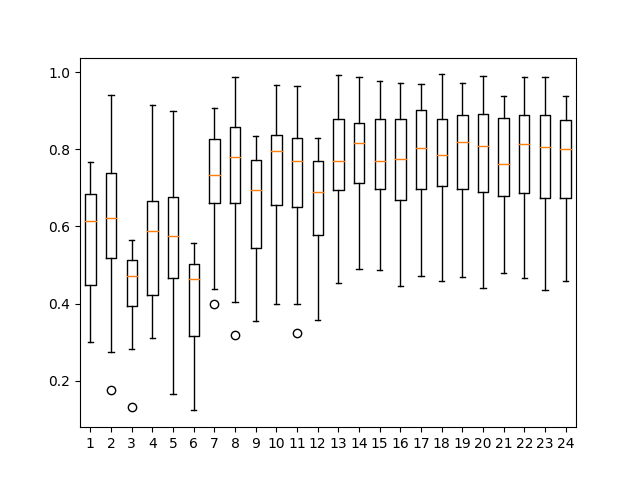
\includegraphics[scale=0.8]{kappa_medium_all.png}

\caption{\emph{Kappa} + reducción de las variaciones de las metaheurísticas para los conjuntos medianos}
\label{medium-kap-all}
\end{figure}

Los \emph{boxplots} que van desde el número 13 hasta el 18 confirman que todas las variantes de MA presentan valores similares. Los p-valores de la tabla \ref{wilcox-MA-med} en el anexo A muestran que todas las variantes de MA son estadísticamente similares en \emph{accuracy} + reducción y \emph{kappa} + reducción

Los \emph{boxpĺots} que van desde el 19 hasta el 24 muestran similitud entre las variantes de CHC. Al evaluar los p-valores de la tabla \ref{wilcox-CHC-med} del anexo A se tiene que CHC, CNN-CHC, ENN-CHC y RSS-CHC son estadísticamente similares, mientras que CNN-RSS-CHC y ENN-RSS-CHC son distintos al resto; esto es porque presentan niveles más bajo de reducción.

De las figuras \ref{small-accu-all} y \ref{small-kap-all} también se puede apreciar que las variantes de MA y las de CHC presentan valores similares. Los resultados de la prueba \emph{Wilcoxon} (ver tabla \ref{wilcox-best-med} en el anexo A) para CNN-MA y CHC muestran p-valores iguales a 6.292e-01 para \emph{accuracy} + reducción y 5.197e-01 para \emph{kappa} + reducción, lo que implica que ambos algoritmos son estadísticamente similares.

Como la diferencia entre CNN-MA y CHC es el tiempo de cómputo, se tiene que CHC con población inicial aleatoria presenta los tiempos más cortos y por lo tanto es la mejor metaheurística para resolver el problema de selección de prototipos sobre conjuntos medianos.


\subsubsection{Conjuntos Grandes}

En esta sección se estudia el comportamiento de las variaciones de GGA, SSGA, MA y CHC al resolver el problema de selección de instancias sobre conjuntos grandes. El objetivo es determinar cuál algoritmo presenta los mejores niveles de \emph{accuracy, kappa} y reducción. Además, se estudia el tiempo que requiere cada algoritmo en dar una solución, con lo que se busca evaluar si hay una buena relación entre tiempo y calidad de los resultados.

\begin{table}[h!]
\centering
\begin{tabular}{l c c c c c c}
\hline
\multirow{2}{*}{\textsc{Algoritmo}}
	& \multicolumn{2}{c}{\textsc{Accuracy}}
	& \multicolumn{2}{c}{\textsc{Kappa}}
	& \textsc{Reducción}
	& \textsc{Tiempo (seg)} \\
	& Training & Test
	& Training & Test \\ 
\hline
\hline

GGA         & 0.9316 & 0.8644 & 0.7994 & 0.6014 & 0.5050 & 672.0273 \\
CNN-GGA     & 0.7106 & 0.6431 & 0.4478 & 0.3094 & 0.8409 & 1568.8913 \\
ENN-GGA     & 0.9357 & 0.8890 & 0.7944 & 0.6453 & 0.1502 & 718.0400 \\
\textbf{RSS-GGA}     & \textbf{0.9150} & \textbf{0.8719} & \textbf{0.7227} & \textbf{0.5821} & \textbf{0.7083} & \textbf{1197.0505} \\
CNN-RSS-GGA & 0.9455 & 0.8588 & 0.8410 & 0.5885 & 0.6089 & 2646.6438 \\
ENN-RSS-GGA & 0.9574 & 0.8798 & 0.8669 & 0.6238 & 0.1025 & 1703.4263 \\

\hline

SSGA & 0.8911 & 0.8743 & 0.6953 & 0.6201 & 0.8056 & 27.6637 \\
CNN-SSGA & 0.8897 & 0.8512 & 0.7002 & 0.5939 & 0.8807 & 90.1004 \\
ENN-SSGA & 0.9097 & 0.8892 & 0.7113 & 0.6441 & 0.6823 & 34.9024 \\
\textbf{RSS-SSGA} & \textbf{0.8968} & \textbf{0.8826} & \textbf{0.6743} & \textbf{0.6271} & \textbf{0.8927} & \textbf{57.7995} \\
CNN-RSS-SSGA & 0.9002 & 0.8634 & 0.7140 & 0.6069 & 0.8434 & 99.1629 \\
ENN-RSS-SSGA & 0.9112 & 0.8805 & 0.7245 & 0.6272 & 0.6668 & 78.5967 \\

\hline

\textbf{MA}   & \textbf{0.8904} & \textbf{0.8999} & \textbf{0.6499} & \textbf{0.6510} & \textbf{0.9973} & \textbf{256.1432} \\
CNN-MA & 0.8925 & 0.8926 & 0.6360 & 0.6341 & 0.9884 & 612.7902 \\
ENN-MA & 0.8807 & 0.8902 & 0.6072 & 0.6145 & 0.9976 & 288.6525 \\
RSS-MA & 0.9000 & 0.9002 & 0.6347 & 0.6343 & 0.9746 & 527.9115 \\
CNN-RSS-MA & 0.8857 & 0.8951 & 0.6176 & 0.6160 & 0.9707 & 960.3951 \\
ENN-RSS-MA & 0.8746 & 0.8912 & 0.6292 & 0.6386 & 0.9969 & 443.0003 \\

\hline

\textbf{CHC}  & \textbf{0.8961} & \textbf{0.8934} & \textbf{0.6614} & \textbf{0.6506} & \textbf{0.9615} & \textbf{16.8665} \\
CNN-CHC & 0.8903 & 0.8871 & 0.6554 & 0.6437 & 0.9771 & 38.3314 \\
ENN-CHC & 0.8993 & 0.8964 & 0.6746 & 0.6631 & 0.9233 & 27.3520 \\
RSS-CHC & 0.8972 & 0.8962 & 0.6591 & 0.6526 & 0.9819 & 41.1142 \\
CNN-RSS-CHC & 0.8945 & 0.8910 & 0.8945 & 0.6435 & 0.9719 & 50.5800 \\
ENN-RSS-CHC & 0.8975 & 0.8922 & 0.6721 & 0.6532 & 0.9099 & 47.4006 \\

\hline
\end{tabular}
\caption{Promedios de las distintas variaciones de cada metaheurística para los conjuntos grandes}
\label{grande-all}
\end{table}

Al estudiar los resultados obtenidos en la tabla \ref{grande-all}, se pueden destacar los siguientes aspectos observados de las variaciones de GGA:

\begin{itemize}

\item RSS-GGA, ENN-GGA y ENN-RSS-GGA presentan los mejores niveles de \emph{accuracy}. 

\item ENN-GGA y ENN-RSS-GGA presentan los mejores niveles de \emph{kappa}.

\item CNN-GGA presenta los peores porcentajes de \emph{accuracy y kappa}. 

\item CNN-GGA y RSS-GGA presentan las mejores tasas de reducción.

\item ENN-GGA y ENN-RSS-GGA presentan las peores tasas de reducción.

\item ENN-GGA y RSS-GGA son las variaciones, excluyendo a GGA, que menos tiempo toman en dar un resultado.

\end{itemize}

De las observaciones anteriores se puede concluir que RSS-GGA es la mejor variación de GGA; esto se debe a que presenta el mejor balance entre \emph{accuracy, kappa} y reducción. Cabe destacar que RSS-GGA obtiene una tasa de reducción 20.33\% mayor que GGA sin comprometer sus niveles de \emph{accuracy y kappa}, lo cual justifica el costo adicional de tiempo que conlleva utilizar RSS.

Al pasar a los resultados obtenidos para las variaciones de SSGA, se puede observar:

\begin{itemize}

\item RSS-SSGA, ENN-SSGA y ENN-RSS-SSGA presentan los mejores valores para \emph{accuracy y kappa}.

\item RSS-SSGA y CNN-SSGA presentan las tasas de reducción más alta.

\item Los mejores tiempos entre las variantes que usan heurísticas son los obtenidos por ENN-SSGA y RSS-SSGA. Ambas variaciones presentan tiempos por debajo del minuto.

\end{itemize}

De las consideraciones anteriores, se puede concluir que RSS-SSGA es la mejor variación de SSGA, ya que presenta la mayor tasa de reducción: 8.71\% por encima de SSGA con población inicial aleatoria, a la vez que mantiene buenos niveles de \emph{accuracy y kappa}, razones que justifican el tiempo adicional de cómputo.

Al evaluar los resultados obtenidos por las variaciones de MA y CHC, se observa:

\begin{itemize}

\item Todas las variaciones presentan valores similares de \emph{accuracy y kappa}.

\item Todas las variaciones presentan tasas de reducción similares.

\end{itemize}

De las observaciones anteriores se concluye que MA y CHC son metaheurísticas capaces de obtener resultados consistentes independientemente de la población inicial que utilicen. Por lo tanto el uso de heurísticas no conlleva a un beneficio real y sólo aumenta el tiempo de cómputo, razón por la cual MA y CHC con población incial aleatoria son las mejores varientes de sus respectivas metaheurísticas.

Al comparar todas las metaheurísticas, se tiene que las variantes de MA y CHC presentan los mejores valores en \emph{accuracy, kappa} y reducción. Al contrastar MA con CHC se tiene que presentan valores de \emph{accuracy y kappa} muy similares, la diferencia está en la tasa de reducción, donde MA supera en 3.58\% a CHC. Sin embargo, si se toma en cuenta que MA tarda 15 veces más en regresar un resultado y que CHC es la metaheurística más rápida; se puede concluir que CHC es la mejor metaheurística para resolver el problema de selección de prototipos sobre conjuntos grandes.